\documentclass[ignorenonframetext,]{beamer}
\setbeamertemplate{caption}[numbered]
\setbeamertemplate{caption label separator}{: }
\setbeamercolor{caption name}{fg=normal text.fg}
\beamertemplatenavigationsymbolsempty
\usepackage{lmodern}
\usepackage{amssymb,amsmath}
\usepackage{ifxetex,ifluatex}
\usepackage{fixltx2e} % provides \textsubscript
\ifnum 0\ifxetex 1\fi\ifluatex 1\fi=0 % if pdftex
  \usepackage[T1]{fontenc}
  \usepackage[utf8]{inputenc}
\else % if luatex or xelatex
  \ifxetex
    \usepackage{mathspec}
  \else
    \usepackage{fontspec}
  \fi
  \defaultfontfeatures{Ligatures=TeX,Scale=MatchLowercase}
\fi
\usetheme[]{Darmstadt}
\usefonttheme{structurebold}
% use upquote if available, for straight quotes in verbatim environments
\IfFileExists{upquote.sty}{\usepackage{upquote}}{}
% use microtype if available
\IfFileExists{microtype.sty}{%
\usepackage{microtype}
\UseMicrotypeSet[protrusion]{basicmath} % disable protrusion for tt fonts
}{}
\newif\ifbibliography
\hypersetup{
            pdftitle={Progrmación en R-Introducción},
            pdfauthor={Santiago Lozano},
            pdfborder={0 0 0},
            breaklinks=true}
\urlstyle{same}  % don't use monospace font for urls
\usepackage{graphicx,grffile}
\makeatletter
\def\maxwidth{\ifdim\Gin@nat@width>\linewidth\linewidth\else\Gin@nat@width\fi}
\def\maxheight{\ifdim\Gin@nat@height>\textheight0.8\textheight\else\Gin@nat@height\fi}
\makeatother
% Scale images if necessary, so that they will not overflow the page
% margins by default, and it is still possible to overwrite the defaults
% using explicit options in \includegraphics[width, height, ...]{}
\setkeys{Gin}{width=\maxwidth,height=\maxheight,keepaspectratio}

% Prevent slide breaks in the middle of a paragraph:
\widowpenalties 1 10000
\raggedbottom

\AtBeginPart{
  \let\insertpartnumber\relax
  \let\partname\relax
  \frame{\partpage}
}
\AtBeginSection{
  \ifbibliography
  \else
    \let\insertsectionnumber\relax
    \let\sectionname\relax
    \frame{\sectionpage}
  \fi
}
\AtBeginSubsection{
  \let\insertsubsectionnumber\relax
  \let\subsectionname\relax
  \frame{\subsectionpage}
}

\setlength{\parindent}{0pt}
\setlength{\parskip}{6pt plus 2pt minus 1pt}
\setlength{\emergencystretch}{3em}  % prevent overfull lines
\providecommand{\tightlist}{%
  \setlength{\itemsep}{0pt}\setlength{\parskip}{0pt}}
\setcounter{secnumdepth}{0}

\title{Progrmación en R-Introducción}
\author{Santiago Lozano}
\date{11 de enero de 2020}

\begin{document}
\frame{\titlepage}

\begin{frame}{La Máquina Universal}

\begin{itemize}
\item
  ¿Qué es exactamente una computadora?¿Cómo puede un dispositivo
  realizar gran cantidad de diferentes tareas?
\item
  Un computador moderno puede definirse como ``una máquina que almacena
  y manipula información bajo el control de programas cambiables''
\end{itemize}

\end{frame}

\begin{frame}{La Máquina Universal}

\begin{itemize}
\item
  Esta definición puede ser vista desde dos elementos claves.

  \begin{itemize}
  \item
    Las computadoras son dispositivos para manipular información (poner
    información y transformarla en nueva )

    \begin{itemize}
    \tightlist
    \item
      Los computadores no son solo máquinas que manipulan información
      (Calculadora, Bomba de Gasolina), no son computadoras pues están
      hechas para realizar una simple y específica tarea
    \end{itemize}
  \end{itemize}
\end{itemize}

\end{frame}

\begin{frame}[fragile]{La Máquina Universal}

\begin{verbatim}
- Las computadoras operan bajo el control de un       programa cambiable

    - Programa Computacional: Es un detallado,            paso a paso conjunto de intrucciones que            dicen a un computador exactamente que               hacer, si se cambia el programa, se cambia           el conjunto de acciones y se realiza una            tarea diferente, la máquina es la misma             pero el programa controla los cambios en            la máquina
\end{verbatim}

\end{frame}

\begin{frame}[fragile]{Including Plots}

You can also embed plots, for example:

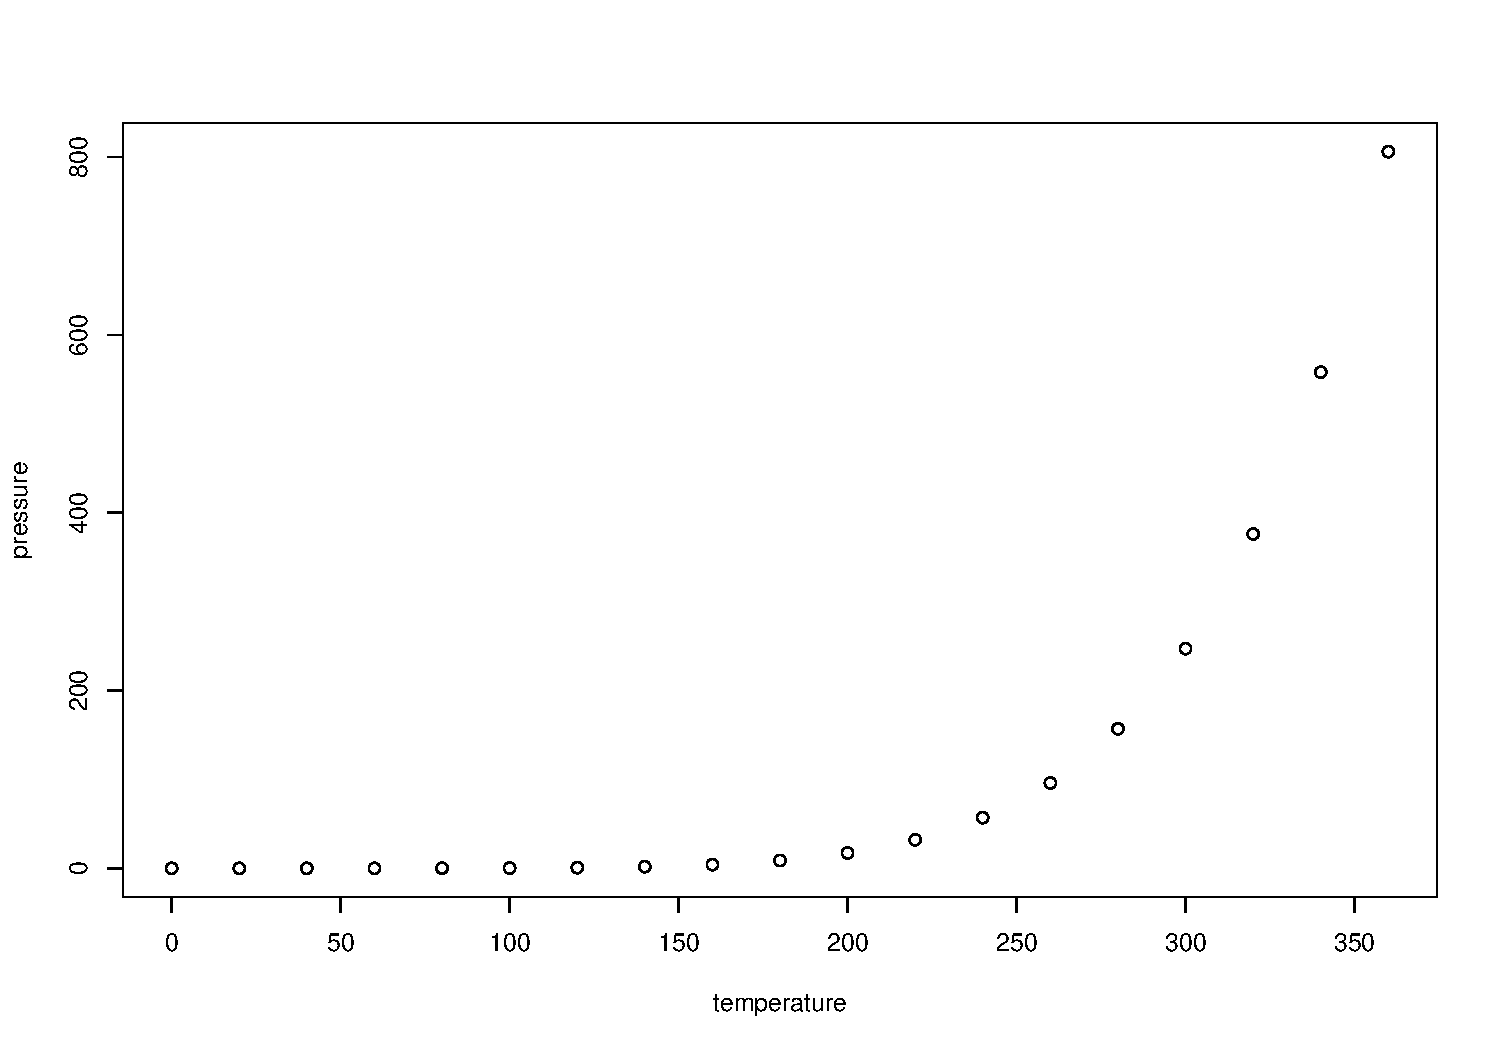
\includegraphics{PR01-Introducción_files/figure-beamer/pressure-1.pdf}

Note that the \texttt{echo\ =\ FALSE} parameter was added to the code
chunk to prevent printing of the R code that generated the plot.

\end{frame}

\end{document}
